% !Mode:: "TeX:UTF-8"

\BiChapter{密集热点区域无线网络的优化}{UDN optimization}

根据第三章的分析,在不采用任何干扰管理和协调算法的情况下,网络中能达到正常工作的信干噪比的用户占总共的用户量的百分比很低。
从而导致了反应网络中所有用户有效性的平均的性能的单位面积谱效率也很低。
因此需要设计一种干扰管理和协调算法提升网络的性能。

本章从两个角度进行分析,即将分两步进行干扰管理和协调,第一步对小区中的微基站进行分簇,从而达到边缘用户减少,
第二步对每个簇中的基站采用~CRAN~网络架构进行联合,由于~CRAN~架构可以将不同微基站的基带信号传输至云化的~BBU~池进行统筹处理。
在~BBU~池侧,可以采用联合传输预编码的方法将发送给不同用户的信息在空域上相互正交,从而达到干扰消除的目的。
\BiSection{密集热点区域无线网络的干扰管理算法的架构}{algorithm construction}
根据图~\ref{e_capacity_show}~显示的结果,在小区中心的用户,收到的干扰较小,遍历容量较好,能达到正常通信的遍历容量需求。
小区边缘的用户的遍历容量较差,反应了小区边缘收到的干扰较为强烈,
接收信干噪比较低,处于边缘的终端出现中断的概率很大,因此要想办法去让边缘用户的性能提升,从而降低网络的中断概率,提高网络覆盖率。

联合传输技术是伴随第四代移动通信~(4G)~提出的一个关键技术。其主要的思想是以用户为中心,将基站联合起来,进行协作,共同对用户进行服务。
由于基站间相互联合共同服务区域内的用户用户,
处在基站边缘的用户的干扰功率也能被用户利用成为有用的接收功率,从而使得边缘用户的有效性大大提升。
联合传输的示意图如图~\ref{CoMP}~所示,在图中,网络由用于处理数字信号的BBU池,用户传输信号的微基站和前向回程链路组成。
传送给用户的信息首先通过BBU池进行数据处理,在通过前向回程链路传输到基站端,由于采用了干扰消除算法,因此两个基站传送给用户的信息均为用户可以利用的有效信号,
实现两个基站联合传输共同服务区域内的用户的目的。
\begin{figure}[htbp]
\centering
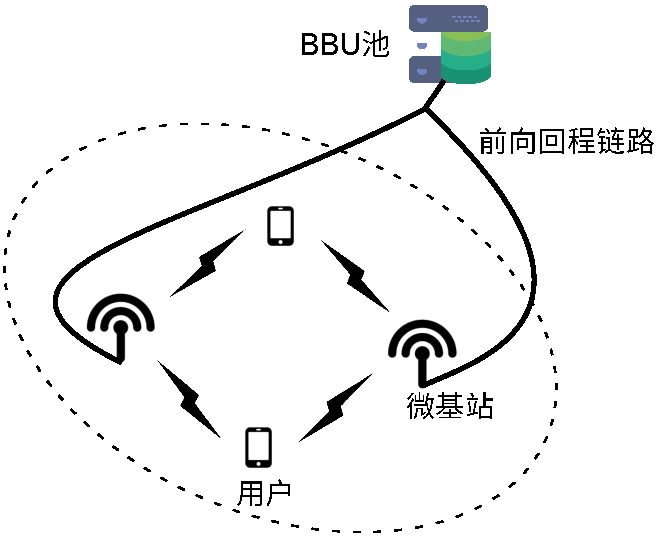
\includegraphics[width = 0.62\textwidth]{CoMP.pdf}
\caption{联合传输网络架构示意图}\vspace{-0.5em}
\label{CoMP}
\end{figure}

在第三章中,定义了网络的网络中基站的拓扑结构,用户的统计特性,信道的基本模型。
即在面积为~$\mathcal{A}$~的区域中,基站的分布~$\Phi$~是一次泊松点过程的实现,
其密度参数为~$\lambda_s$,基站的个数为~n~个,用户在网络中的分布在微基站附近的分布更多,
随着距离基站越来越远,用户出现的概率越小。
假设用户服从以基站位置为均值的混合二维高斯分布,定义物理量~$\sigma$~表示用户的发散程度,量纲为米。
其中~$\sigma$~表示混合二维高斯分布的标准差。
在之前的分析中,由于没有采用多用户联合传输技术,因此所有基站的功率假设是等功率的,
而采用了联合传输以后,可以对所有的基站进行统一的调度,因此网络可以进一步通过功率控制的方法进行优化。
现假设基站~$S_i$~的最大发射功率为~$P$。
除此之外,本文采用的多用户联合传输中,为了进行干扰管理,采用预编码的技术进行干扰消除,预编码矩阵为~$\mathbf{W}$。
用户~$U_j$~接收到基站~$S_i$~的接收功率受到基站~$S_i$~的最大的发射功率~$P$,预编码矩阵~$\mathbf{W}$,描述信道的大尺度衰落的信道衰减系数~$\alpha$,
描述瑞利信道的随机变量~$h$决定。

 假设采用~BPSK~调制方式,在小区中一共有~$k$~个用户~$n$~个基站,
 基站发射给用户的信息为~$\mathbf{q}=\{q_1,q_2,\dots,q_j,\dots,q_k\}$,
 其中~$q_j\in\{1,-1\}$~表示用户~$U_j$~想要接收到的信号。
 在进行预编码之前需要首先要确定每个用户所需要分配的功率。
 在进行功率分配后,待发射的信号~$\mathbf{x} = \{x_1,x_2,\dots,x_j,\dots,x_k\} = \{p_1 q_1,p_2 q_2,\dots,p_j q_j,\dots,p_k q_k\}$。
 其中为~$\mathbf{p}=\{p_1,p_2,\dots,p_j,\dots,p_k\}$~为功率分配权重。
 因此用户~$j$~分配到的功率的值为~${p_j}^2$~

 预编码矩阵为~${\mathbf{W}=\{w_{ij}\}}_{n\times k}$。
 其中~$w_{ij}$~表示第~$j$~个用户所发送的信息在第~$i$~个基站所占的权值。则基站的发射信号向量~$\mathbf{s}$可表示为:
 \begin{equation}\label{send_s}
   \mathbf{s}=\mathbf{W} \mathbf{x}
 \end{equation}
其中~$\mathbf{x}$~为发射信号的向量,$\mathbf{W}$~为预编码矩阵,
可将预编码矩阵~$\mathbf{W}$~表示为~$n\times 1$~的分块矩阵
~$\mathbf{W}=\{\mathbf{w}_1, \mathbf{w}_2,\cdots,\mathbf{w}_k\}^{\mathrm{T}}$。
在联合传输的过程中,所有的基站共享用户的发送信息和信道状态信息,
以得到状态信息作为参数,得到的预编码矩阵,即可以对网络的有效性进行优化,
通过预编码矩阵修改发送每个用户信息的权重,
将加权后的信号交由基站进行发送。

基站发送的信号受到大尺度衰落和小尺度衰落的影响。
定义系数矩阵~$\mathbf{G}=\{g_{ij}\}_{k\times n}$,
其中~$g_{ij}\in\mathbb{R}$,$g_{ij} = h_{ij}R_{ij}^{-\alpha}$,
其中~$h_{ij}$~和~$R_{ij}$~分别表示基站~$S_i$~和用户~$U_j$~之间的信道系数和距离。
用户的接收信号向量~$\mathbf{y}$~为:
\begin{equation}\label{received_y}
  \mathbf{y} = \mathbf{Gs} + \mathbf{z}
\end{equation}
其中~$\mathbf{G}$~为信道的系数矩阵,$z\in \mathbb{R}$~为加性高斯白噪声,噪声的功率谱密度为~$N_0$。

若采用基于~ZFBF~的多用户联合传输技术,则预编码矩阵~$\mathbf{W}$~为:
\begin{equation}\label{precode_w}
  \mathbf{W} = \mathbf{G}^{\mathrm{T}}(\mathbf{G}\mathbf{G}^{\mathrm{T}})^{-1}
\end{equation}
其中~$\mathrm{T}$~表示转置,即采用基于~ZFBF~的多用户联合传输技术的情况下,
预编码矩阵为信道系数矩阵的广义逆。

将式~(\ref{send_s})~和式~(\ref{precode_w})~带入到式~(\ref{received_y})~中,
可以得到接收信号关于发送信号~$\mathbf{x}$~和噪声~$\mathbf{z}$~的表达式:
\begin{equation}
  \mathbf{y} = \mathbf{x} + \mathbf{z}
\end{equation}

由于干扰通过基于~ZFBF~的多用户联合传输技术已将消除掉了,
因此用户的接收信干噪比与信噪比相同,用户~$j$~的信干噪比~$\gamma_{j}$~如式~(\ref{gamma_r})~所示:
\begin{equation}\label{gamma_r}
  \gamma_j = \frac{{x_j}^2}{N_0}= \frac{{p_j}^2}{N_0}
\end{equation}
用户~$U_j$~的容量的表达式为:
\begin{equation}
  R_j = \log_2(1+\gamma_j)
\end{equation}
若要提升网络的覆盖率,则需要让所有的用户都能达到较高的信噪比,则目标函数就会发生相应的变化,
为了反应网络的覆盖率这一性能,需采用最大最小的目标函数,及最大化最小的用户的容量,
每个基站均要满足功率约束条件,且为每个用户分配的功率的系数不能为负值。
优化问题的表达式如式~(\ref{maxmin})~所示:
\begin{equation}\label{maxmin}
  \begin{aligned}
&\max\,\, \min\{\gamma_1, \gamma_2, \cdots, \gamma_k\}\\
&s.t.\quad
\begin{cases}
0\leq(\mathbf{w}_i\mathbf{x})^2\leq P, & j=1,2,3,\cdots,k, \\
p_j \geq 0, & j=1,2,3,\cdots,k.
\end{cases}
\end{aligned}
\end{equation}

为了得到更高的单位面积频谱效率,需要让区域内的所有用户的容量的和达到最大值,
但是每个基站的发送功率不能超过基站所能提供的功率的门限~$P$。
基于~ZFBF~的多用户联合传输技术,要得到最优的单位面积频谱效率,需要解决如下的优化问题:
\begin{equation}\label{opt_R}
  \begin{aligned}
&\max\,\, R=\sum_{j=1}^n \gamma_j\\
&s.t.\quad
\begin{cases}
0\leq(\mathbf{w}_i\mathbf{x})^2\leq P, & j=1,2,3,\cdots,k, \\
p_j \geq 0, & j=1,2,3,\cdots,k.
\end{cases}
\end{aligned}
\end{equation}

联合传输可以统筹信道状态信息,用户的发送信息,可以采用多基站写作的方法对干扰进行抑制,
达到提升网络性能的目的。
不仅如此,由于基站可以通过一个中心控制器进行统一的调度,可以选取不同的目标函数,
使网络的某些特定性能,如覆盖率,单位面积频谱效率达到最优,实现网络优化的目的。

虽然联合传输可以技术可以提升边缘用户的通信性能,提高覆盖率,
提升网络的和速率,最大化单位面积频谱效率,
但是联合传输技术并不能直接用于密集热点区域无线网络当中,在密集热点区域无线网络中,
区域内的基站较为密集,基站的分布是不均匀的,
且一般情况下数量较多,如果将区域内的所有基站全部都联合在一起,系统的复杂度很高,实现难度太大。

为改进联合传输技术,使其不但能增加使处在服务区域边缘的用户的传输可靠性,提升网络的性能,又能有较低的复杂度。
本文提出的干扰管理算法分为两个步骤,首先,对小区中的微基站进行分簇,将簇内的基站整体作为协作集,共享信道的发送信息与信道状态信息。
然后再对每个簇中的基站采用~CRAN~网络架构进行联合,对同一个簇中的用户采用联合传输策略,
将簇内发送给各个用户的有用信号在空域上尽可能的正交,
增强发送给用户的有用信号,
抑制用户接收到的干扰,
达到增加网络的覆盖率,提升网络的区域面积频谱效率的目的。
网络的示意图如图~\ref{CoMP_cluster}~所示:
在图中,将小区内的~5~个基站分成了三个簇,分别为簇~A,簇~B和簇~C,当簇内含有多个基站时多用户联合传输的网络架构,
通过云服务器对发送的信号进行集中的数字信号处理。
对簇内采用干扰管理和协调算法,但不同簇的基站之间会产生簇间干扰。

\BiSection{密集热点区域无线网络的基站分簇}{clustering of basestation in UDN}

本小节对密集热点区域无线网络的基站的分簇算法进行研究,提出基于深度优先搜索的网络中微基站分簇算法。
将距离相聚过近的基站进行联合,
消除由基站过近导致的强烈的干扰,
也避免由于基站之间相距过近而导致边缘用户较多的情况发生。

本节将深度优先搜索算法和~k~-~均值算法应用到网络的分簇当中。下面分别介绍基于上述两种算法的网络分簇方法。
\begin{figure}[htbp]
\centering
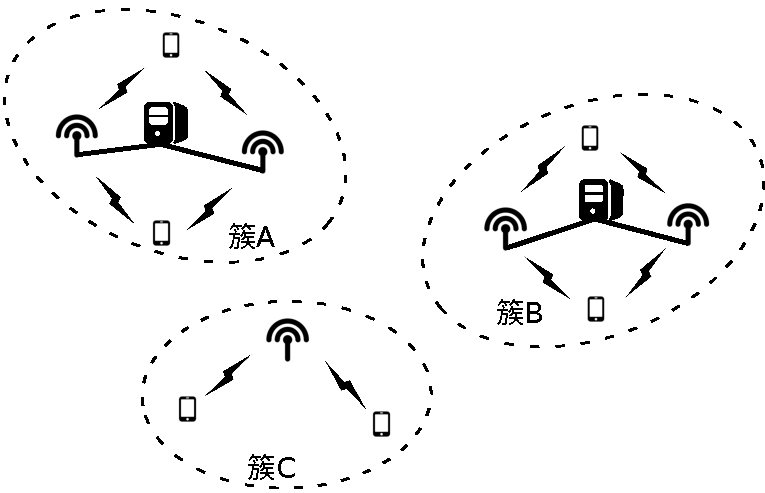
\includegraphics[width = 0.7\textwidth]{CoMP_cluster.pdf}
\caption{密集热点区域无线网络的干扰管理架构示意图}\vspace{-0.5em}
\label{CoMP_cluster}
\end{figure}
\BiSubsection{基于深度优先搜索的微基站分簇算法}{Time diversity}
根据图~\ref{e_capacity_show}~所示,相邻的基站之间如果距离过近,则由于基站之间的干扰强烈,小区中用户的遍历容量性能,
网络的覆盖率和单位面积频谱效率性能将会受到巨大的影响,除此之外,如果两个基站的距离过近,
由于微基站服务的区域用户量需求大,
容量要求高,因此两个基站之间会存在大量的边缘用户,从而极大的影响了系统的性能。

为了避免基站相聚过近而导致的基站之间的干扰强烈,边缘用户过多。
本小节提出了基于深度优先搜索的基站分簇算法。
深度优先搜索算法是计算机科学当中的基础算法,也是图论当中比较经典的算法之一。

下面介绍基于图的深度优先搜索的为基站分簇算法,为了应用按深度优先的搜索,首先需要在将网络中的基站拓扑映射成为一个图结构。
给定区域~$\mathcal{D}$~中的所有基站
~$\mathcal{S}(x,y)=\{S_1(x_1,y_1), S_2(x_2,y_2),\dots,S_i(x_i,y_i)~,\dots,S_n(x_n,y_n)\}$,
其中~$x$,$y$~分别表示基站的横,纵坐标。
对任意的~$i,j\in\{1,2,\dots,n\}$,基站~$S_i$~与基站~$S_j$~之间的距离为~$R_{ij}$,
根据微基站集合~$\mathcal{S}$~和基站之间的距离~$R_{ij}$,$i,j \in\{1,2,\dots,n\}$构造图~$\mathcal{G}$,
其中图~$\mathcal{G}$~的节点集合~$\mathcal{V}=\{v_1,v_2,\dots,v_i,\dots v_n\}$~
为微基站集合~$\mathcal{S}$~的一一映射,即对任意给定的~$i\in\{1,2,\dots,n\}$,
存在映射关系~$S_i \rightarrow v_i$。图~$\mathcal{G}$~的所有边构成的集合~$\mathcal{E}$~
根据微基站之间的距离是否小于门限~$\tau$~决定,即对任意的~$i,j\in\{1,2,\dots,n\}$,若~$R_{ij}<\tau$,
则存在边~$e_{ij}\in\mathcal{E}$,
表示图~$\mathcal{G}$~中存在边~$e_{ij}$~将节点~$v_i$~和节点~$v_j$~连接。
根据图~$\mathcal{G}$~的边集合~$\mathcal{E}$,可以构造邻接矩阵~$\mathbf{A}=\{a_{ij}\}_{n\times n}$,其中
\begin{equation}
a_{ij}=
\begin{cases}
1, & e_{ij}\in \mathcal{E}, \\
0, & e_{ij}\notin \mathcal{E}.
\end{cases}
\end{equation}

在~$\mathcal{G}$~中,定义两个节点~$v_i$~和~$v_j$~是连通的,则从定点~$i$~到定点~$j$~有路径相连。
基于深度优先搜索的基站分簇算法将所有连通的节点划归为一簇,
将图~$\mathcal{G}$~划归为由不同子图构成的不交并,
由于图上的节点和微基站之间有一一映射的关系,
属于同一个子图的节点相互连通。
可将处在同一个子图上的节点对应的基站划分成为一个簇。
即~$\mathcal{S} = \dot{\bigcup\nolimits}_{i=1}^{m}\mathcal{C}_i$,
表示将基站的集合~$S$~分成了~$m$~个子集合,每个集合里的基站构成一簇。
完整的描述如算法~\ref{algorithm_bs_dfs}~所示:


\begin{algorithm}[!htb]
\caption{ 基于深度优先搜索的基站分簇算法 }
\label{algorithm_bs_dfs}
\small
\SetKwProg{Fn}{Function}{}{end}
\KwIn{  $\tau$~;$\mathcal{S}(x,y)$}
\KwOut{ $\mathcal{K}$ }
\Begin
{
    第~1~步:初始化\\
    $\mathbf{A}=\{a_{ij}\}_{n\times n}=\{0\}_{n\times n}$~;
    $c=0$~;
    $\mathcal{K}=\varnothing$~;
    $\mathbf{v}=\{v_i\}_n=\{0\}_n$~\\

    第~2~步:构造邻接矩阵~$\mathbf{A}$:\\
    \For{~$i=1 \ to \ n$,$j=1 ~ to ~ n$~}
    {
          $a_{ij}=(\sqrt{({x_i} - {x_j})^2+(y_i-y_j)^2} < 0~)$  \\
    }
    第~3~步:构造深度优先搜索函数:\\
    \Fn{$DFS$(~$node$~$i$~, $\mathcal{C}_c$~)}
    {
      \For{~$j=1\ to\ n, j \neq i$~}
      {
        \If{~$v_j==0 \ \ and\ \ a_{ij} == 1$~}
        {
          $v_{j}=1$ \\
          $\mathcal{C}_c=\mathcal{C}_c \bigcup~ \{~S_j~\}$\\
          $\emph{DFS(~j~,~}\mathcal{C}_c ~\emph{)}$\\
        }
      }
    }
    第~4~步: 基于深度优先搜索的基站分簇\\
    \For{~$i=1 \ to \ n$~}
    {
      \If{~$v_i == 0$~}{
        $c ~+= 1$ \\
        $\mathcal{C}_c = \{~S_i~\}$\\
        $v_i = 1$\\
        $\emph{DFS(~i~,~}\mathcal{C}_c ~\emph{)}$\\
        $\mathcal{K} = \mathcal{K} \bigcup~ \{~\mathcal{C}_c~\}$\\
      }
    }
}
\end{algorithm}

算法的输入为距离门限~$\tau$和基站的坐标参数~$\mathcal{S}(x,y)$,
算法分为四个步骤执行。

其中第一步为初始化步骤,
将邻接矩阵~$\mathbf{A}$~初始化为~$\mathbf{0}_{n\times n}$,
将网络中微基站簇的个数~$c$~设置为0个,
微基站簇的集合~$\mathcal{K}$~设置为空集~$\varnothing$,
用于标识是否与微基站一一映射的节点是否访问过的向量~$\mathbf{v}$~设置为~$\mathbf{0}_{n\times 1}$,
对应位置为~0~表示未被访问,为~1~表示已经被访问。

算法的第二步为构造邻接矩阵,
对任意的基站~$S_i$~和~$S_j, ~i, ~j \in \{~1,~2,\cdots,~n~\}$,
当基站之间的距离小于门限~$\tau$,则邻接矩阵对应的位置~$a_{ij}=a_{ji}=1$,
否则邻接矩阵对应的位置~$a_{ij}=a_{ji}=0$。

算法的第三步为构造邻接矩阵的深度优先搜索的矩阵,
深度优先搜索用于将与给定的节点~$i$~的所有连通的节点全部搜索出来,构成集合~$\mathcal{C}$~。
首先将节点~$i$~对应的基站~$S_i$~放入集合~$\mathcal{C}$~中,
并将向量~$\mathbf{v}$~中的第~$i$~位~$v_i$~置~1,
接着采用递归的方法依次遍历所有除给定节点~$i$~以外的节点,
如果存在节点~$j$~与给定节点~$i$~相连通且未被遍历,
则将微基站~$S_j$~放入集合~$\mathcal{C}$~中,
并将向量~$\mathbf{v}$~中的第~$j$~位~$v_j$~置~1,
从节点~$j$~开始继续执行按深度搜索的遍历,
直到所有与给定节点~$i$~连通的节点都被找到为止。
通过深度优先搜索函数可以得到网络中的一簇基站。

算法的第四步应用第三步给出的深度优先搜索函数,从~1~到~$n$~依次开始遍历整张图,
如果节点~$i$~未被分簇,通过函数找到与节点~$i$~连通的所有节点作为一簇。
直到所有的节点均被分簇为止。


算法通过给定距离门限,将小于距离门限的所有基站连接在了一起。这些基站共同给所覆盖区域内的用户进行服务。
从而极大的降低了边缘用户的数量,增大了用户所接收到的有用功率,减小了用户接收到的干扰。

但是,由于小区中基站的部署是泊松点过程,因此,小区中的基站的分布并不均匀,
因此可能会出现某个协作集当中的基站过多,
从而可能导致多用户簇内的多用户联合传输的复杂度过高。
不仅如此,由于小区中的微基站采用了以基站为中心的分簇方式。
小区中的服务范围依然存在明显的边界,处在边界上的用户依然会可能会受到比较严重的干扰。


\BiSubsection{基于~k~-~均值的微基站分簇算法}{Time diversity}
K~-~均值算法是人工智能领域常用的一种非监督学习算法\citeup{InfoTheoryInference}。
其是一种基于迭代的统计学习方法,由~Dempster~等人总结提出,
是均方最大(~EM~)算法的一种特例\citeup{statisticslearning}。
算法的主要步骤分为两步,即分配步骤和更新步骤。
功能分别为设定权重矩阵和更新均值点集。
与机器的思考方式不同,人类可以很容易的辨识区域内的物体,并将这些物体分类。
但若要让计算机也可以对空间内的点集进行分簇,
需要采用聚类算法,将簇内基站相距距离较近,并且与簇外基站相距较远,
并且由于算法存在均值,一个簇所划归的区域近似为一个圆形。
k~-~均值算法首先随机生成~k~个点作为均值的初始点,均值点的集合用~$\mathcal{M}$~表示,
$\mathcal{M}=\{~M_1(x_1,y_1),~M_2(x_2,y_2),\dots,~M_k(x_k,y_k)~\}$。
将每个均值附近的点作为一簇,再通过簇内点集迭代出新的均值。
直到算法收敛或迭代次数耗尽为止。

在密集热点区域无线网络覆盖的区域~$\mathcal{D}$~上,
已知微基站的位置坐标集合~$\mathcal{S}(x,y) = \{S_1(x_1,y_1), S_2(x_2,y_2),\dots,S_n(x_n,y_n)\}$。
用~k~-均值算法将点集~$\mathcal{S}(x,y)$~分成~K~个簇~$\mathcal{S} = \dot{\bigcup}_{i=1}^{k} \mathcal{C}_i$。
对任意的~$i\in\{~1,~,2,\dots,~n~\}$,$j\in\{~1,~2,\dots,~k~\}$,
$d(~S_i,~M_j~)$~表示微基站~$S_i$~和均值~$M_j$~之间的距离。算法的描述如算法~\ref{kmeansalgorithm}~所示:
\begin{algorithm}[!htb]
\caption{ 基于~k~-均值聚类的基站分簇算法 }
\label{kmeansalgorithm}
\small
\SetKwProg{Fn}{Function}{}{end}
\KwIn{$k$~;$\mathcal{S}(~x,~y~)$~;$iter$}
\KwOut{$\mathcal{M}$}
\Begin
{
    第1步:初始化\\
    随机生成~k~个坐标~$\mathcal{M}=\{~M_1,~M_2,\cdots,~M_k~\}$~构成均值点集;\\
    生成权值矩阵~$\mathbf{C}=\{~0~\}_{n\times k}$~;\\
    迭代次数~$count=0$~\\

    第2步:~k~-~均值算法:\\
    \While{~$count++ < ~iter$~}
    {
      步骤~2.1:设定权重矩阵\\
      $\mathbf{C}=\{~c_{ij}~\}_{n\times k}=\{~0~\}_{n\times k}$\\
      \For{~$i=1 \ to \ n$~}
      {
        $\hat{j}=\arg\min\limits_{j} ~d(~S_i,~M_j~)$ \\
        $c_{i\hat{j}}=1$  \\
      }

      步骤~2.2~:均值点集更新:\\
      \For{~$j=1 \ to \ k$~}
      {
        $C_j = \sum_{i=1}^n c_{ij}$  \\
        $M_j(~x_j, y_j~) = \frac{\sum_{i=1}^{n} c_{ij} S_i(~x_i,~y_i~)}{C_j}$  \\
      }
    }
}
\end{algorithm}

首先输入基站分簇的簇的个数~k~,微基站的坐标~$\mathcal{S}(~x,y~)$,迭代次数~$iter$。
算法主要分为两步,第~1~步为初始化部分,随机生成~k~个点作为均值点的初值,
权重矩阵~$\mathbf{C}$~设定为全~0~矩阵,设定迭代次数~$count$~为~0。
算法的第~2~步为~k~-~均值算法的实现,是一个迭代的过程,迭代的次数为~$iter$~次。
迭代的过程分为两个子步骤,子步骤~2.1~找遍历所有的微基站,找到距离微基站最近的均值点,
将权重矩阵~$\mathbf{C}$~相应的位置置~1。
子步骤~2.2~用得到的权值矩阵~$\mathbf{W}$~
对基站的坐标~$\mathcal{S}(~x,~y~)$~进行权值更新得到新的均值集合~$\mathcal{M}$。

基于~k~-均值算法的聚类可以对基站进行分簇,与基于深度搜索算法的基站分簇不同,
基于~k~-~均值算法的基站分簇将区域内的基站均匀的分配到~k~个簇当中,
每个区域的大小也近似相同,是一种有效的基站分簇算法。
并且基于~k~-~均值的基站分簇算法可以的到网络的中心,
簇的大致位置可以通过均值的信息反映出来。

基于~k~-~均值算法的基站分簇需要预先设置好簇的个数,
为了得到最优的簇的个数,
需要进行多次试验。
不仅如此,算法需要通过迭代实现分簇,算法的复杂度较高。
由于算法并不是依据基站之间的关系进行分簇,因此也没有利用基站之间的拓扑结构这一信息。

\BiSection{密集热点区域无线网络的簇内干扰消除与优化}{algorithm construction}

\BiSection{密集热点区域无线网络优化的性能分析}{analysis}
\BiSubsection{网络分簇算法的分析}{cluster}

在第三章,我们给出了网络仿真的网络示意图~\ref{network_show},
对基于深度优先搜索算法的基站分簇算法得到的分簇结果进行仿真,
仿真参数如表~\ref{dfs_show_sim_para}~所示:
\begin{table}[htbp]
\caption{基于深度优先搜索的分簇算法的仿真参数}
\label{dfs_show_sim_para}
\vspace{0.5em}\centering\wuhao
\begin{tabular}{cccc}
\toprule[1.5pt]
参量 & & & 设置 \\
\midrule[0.5pt]
基站的分布~$\Phi$~ & & & 泊松点过程 \\
泊松点过程的密度参数~$\lambda_s$~ & & & ~$0.01~\mathrm{m}^{-2}$~ \\
区域的大小  & & & ~$100\mathrm{m} \times 100 \mathrm{m}$~ \\
基站的个数~$n$~  & & & 100\\
深度搜索的距离门限~$\tau$~ & & & ~$5\mathrm{m}$~\\
\bottomrule[1.5pt]
\end{tabular}
\end{table}

选取的区域的大小为 ~$100\mathrm{m} \times 100 \mathrm{m}$~的正方形的区域,
正方形的区域中的基站的部署为泊松点过程,密度参数为~$\lambda_s=0.01 \mathrm{m}^{-2}$,
距离门限~$\tau=5~\mathrm{m}$。
对生成的这片区域采用基于深度优先搜索的分簇算法,得到的网络示意图如图~\ref{dfs_network_show}~所示:
\begin{figure}[htbp]
\centering
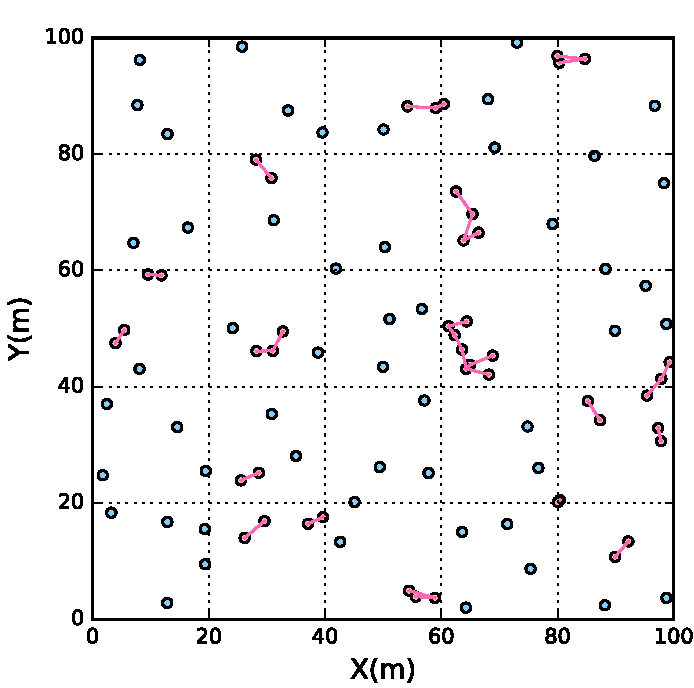
\includegraphics[width = 0.62\textwidth]{dfs_network_show.pdf}
\caption{基于深度优先搜索的分簇算法的效果图}\vspace{-0.5em}
\label{dfs_network_show}
\end{figure}
其中的蓝色的点表示独立的微基站,粉色的点表示使用了多用户联合传输的微基站。
如果微基站的节点之间有一条边相连,则两个基站同属于一个簇。
可以看到,当两个基站的距离~$R_{i,j} < 5$~时,基站就会被连接在一起,共同的归于一个簇。
验证了算法的正确性。
由于密集热点区域的用户具有集中性,因此当两个基站之间的距离过远时,处在边缘的用户更少。
除此之外,基站之间的距离较远,所服务的用户距离干扰基站的距离更远,有效的避免了基站相聚过近的干扰,以及处在边缘的用户的数量过多对性能的影响。

对基于~k~-~均值的基站分簇算法进行仿真
,对一片区域内的的微基站进行分簇,得到分簇结果,
仿真的参数表如表~\ref{kmeans_show_sim_para}所示:
\begin{table}[htbp]
\caption{基于深度优先搜索的分簇算法的仿真参数}
\label{kmeans_show_sim_para}
\vspace{0.5em}\centering\wuhao
\begin{tabular}{cccc}
\toprule[1.5pt]
参量 & & & 设置 \\
\midrule[0.5pt]
基站的分布~$\Phi$~ & & & 泊松点过程 \\
泊松点过程的密度参数~$\lambda_s$~ & & & ~$0.01~\mathrm{m}^{-2}$~ \\
区域的大小  & & & ~$100~\mathrm{m} \times 100~ \mathrm{m}$~ \\
基站的个数~$n$~  & & & 100\\
簇的个数~$k$~ & & & ~$20$~\\
\bottomrule[1.5pt]
\end{tabular}
\end{table}

选取的区域的大小为~$100~\mathrm{m} \times 100~ \mathrm{m}$~的正方形区域,
正方形的区域中的基站部署为泊松点过程,密度参数~$\lambda_s=0.01~m^{-2}$,设置分簇的个数为~$20$~个。
对以泊松点过程生成的基站采用基于~k~-~均值的基站分簇算法,得到的网络示意图如图~\ref{kmeans_network_show}~所示:
\begin{figure}[htbp]
\centering
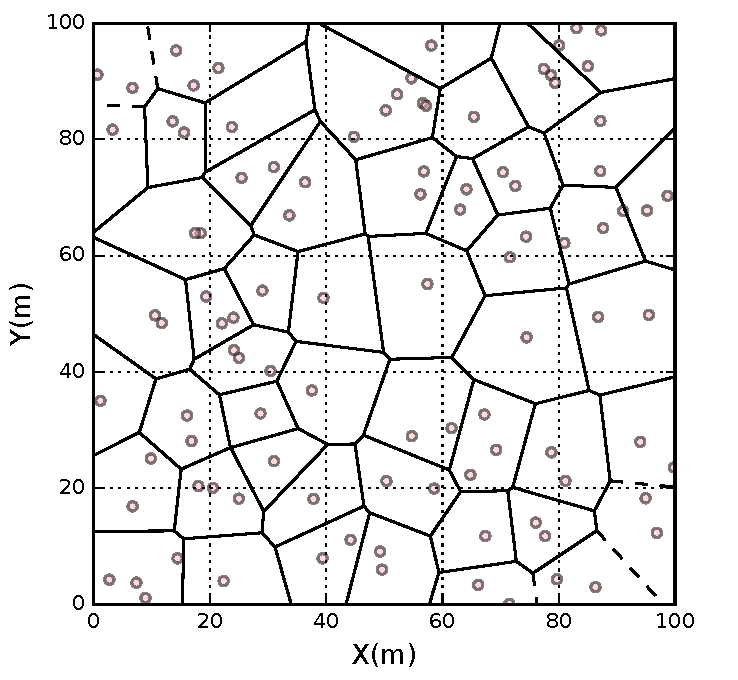
\includegraphics[width = 0.62\textwidth]{kmeans_network_show.pdf}
\caption{基于~k~-~均值的分簇算法的效果图}\vspace{-0.5em}
\label{kmeans_network_show}
\end{figure}
可以看到整个区域被泰森多边形分割,归属于同一个泰森多边形的基站作为一簇,簇内的微基站采用多用户联合传输算法,
多边形内粉色的点表示联合起来的基站。可以看到基站均匀的被分割成了以均值为中心的区域。每个簇内大约有~5~个微基站。
